\chapter[Results and Evaluation]{Results and Evaluation }
\section{Generating the Data}
\vspace{12pt}

For benchmarking and comparing this hybrid network with other networks needs to be done using parameters like Throughput, Network initialization time and latency properties of these networks. According to the literature review, we have done before these are the main matrices that most of the researchers used in order to compare the performance of these networks with each other. Additionally, we are benchmarking the power consumption of these devices in order to get a good understanding of the real-world implications of this network.

\vspace{12pt}
The throughput of the networks was measured with the help of the Linux networking tools wget and Nginx. we hosted an Nginx server on the port 8080 of each device and measured the downloading speeds of each of the devices when using the particular networks. Furthermore, we have taken these measurements multiple times in order to create a more accurate result data set.

\vspace{12pt}
Networking tool Ping was used in conjunction with the bash current system time variable in order to calculate the start-up time of the networks. we wrote a bash script to calculate the time difference from the start time to positive ping response time for the currently enabled device. As the cellular and WIFI networks have almost instantaneous response time we are only considering the hybrid network benchmarks for this metric.

\vspace{12pt}
Network latency of these networks can be easily calculated using the ping commands. To get more accurate results we repeated the experiment many times at different time intervals using different devices.
\clearpage
It was not possible to measure the exact power draw for these networks as we cannot power off most of the default applications in the mobile device. we have used the battery power draw information to calculate the power draw of the system. To get a more accurate result we have taken multiple readings using multiple devices.


\section{Results}


\begin{figure}[H]
    \centering
    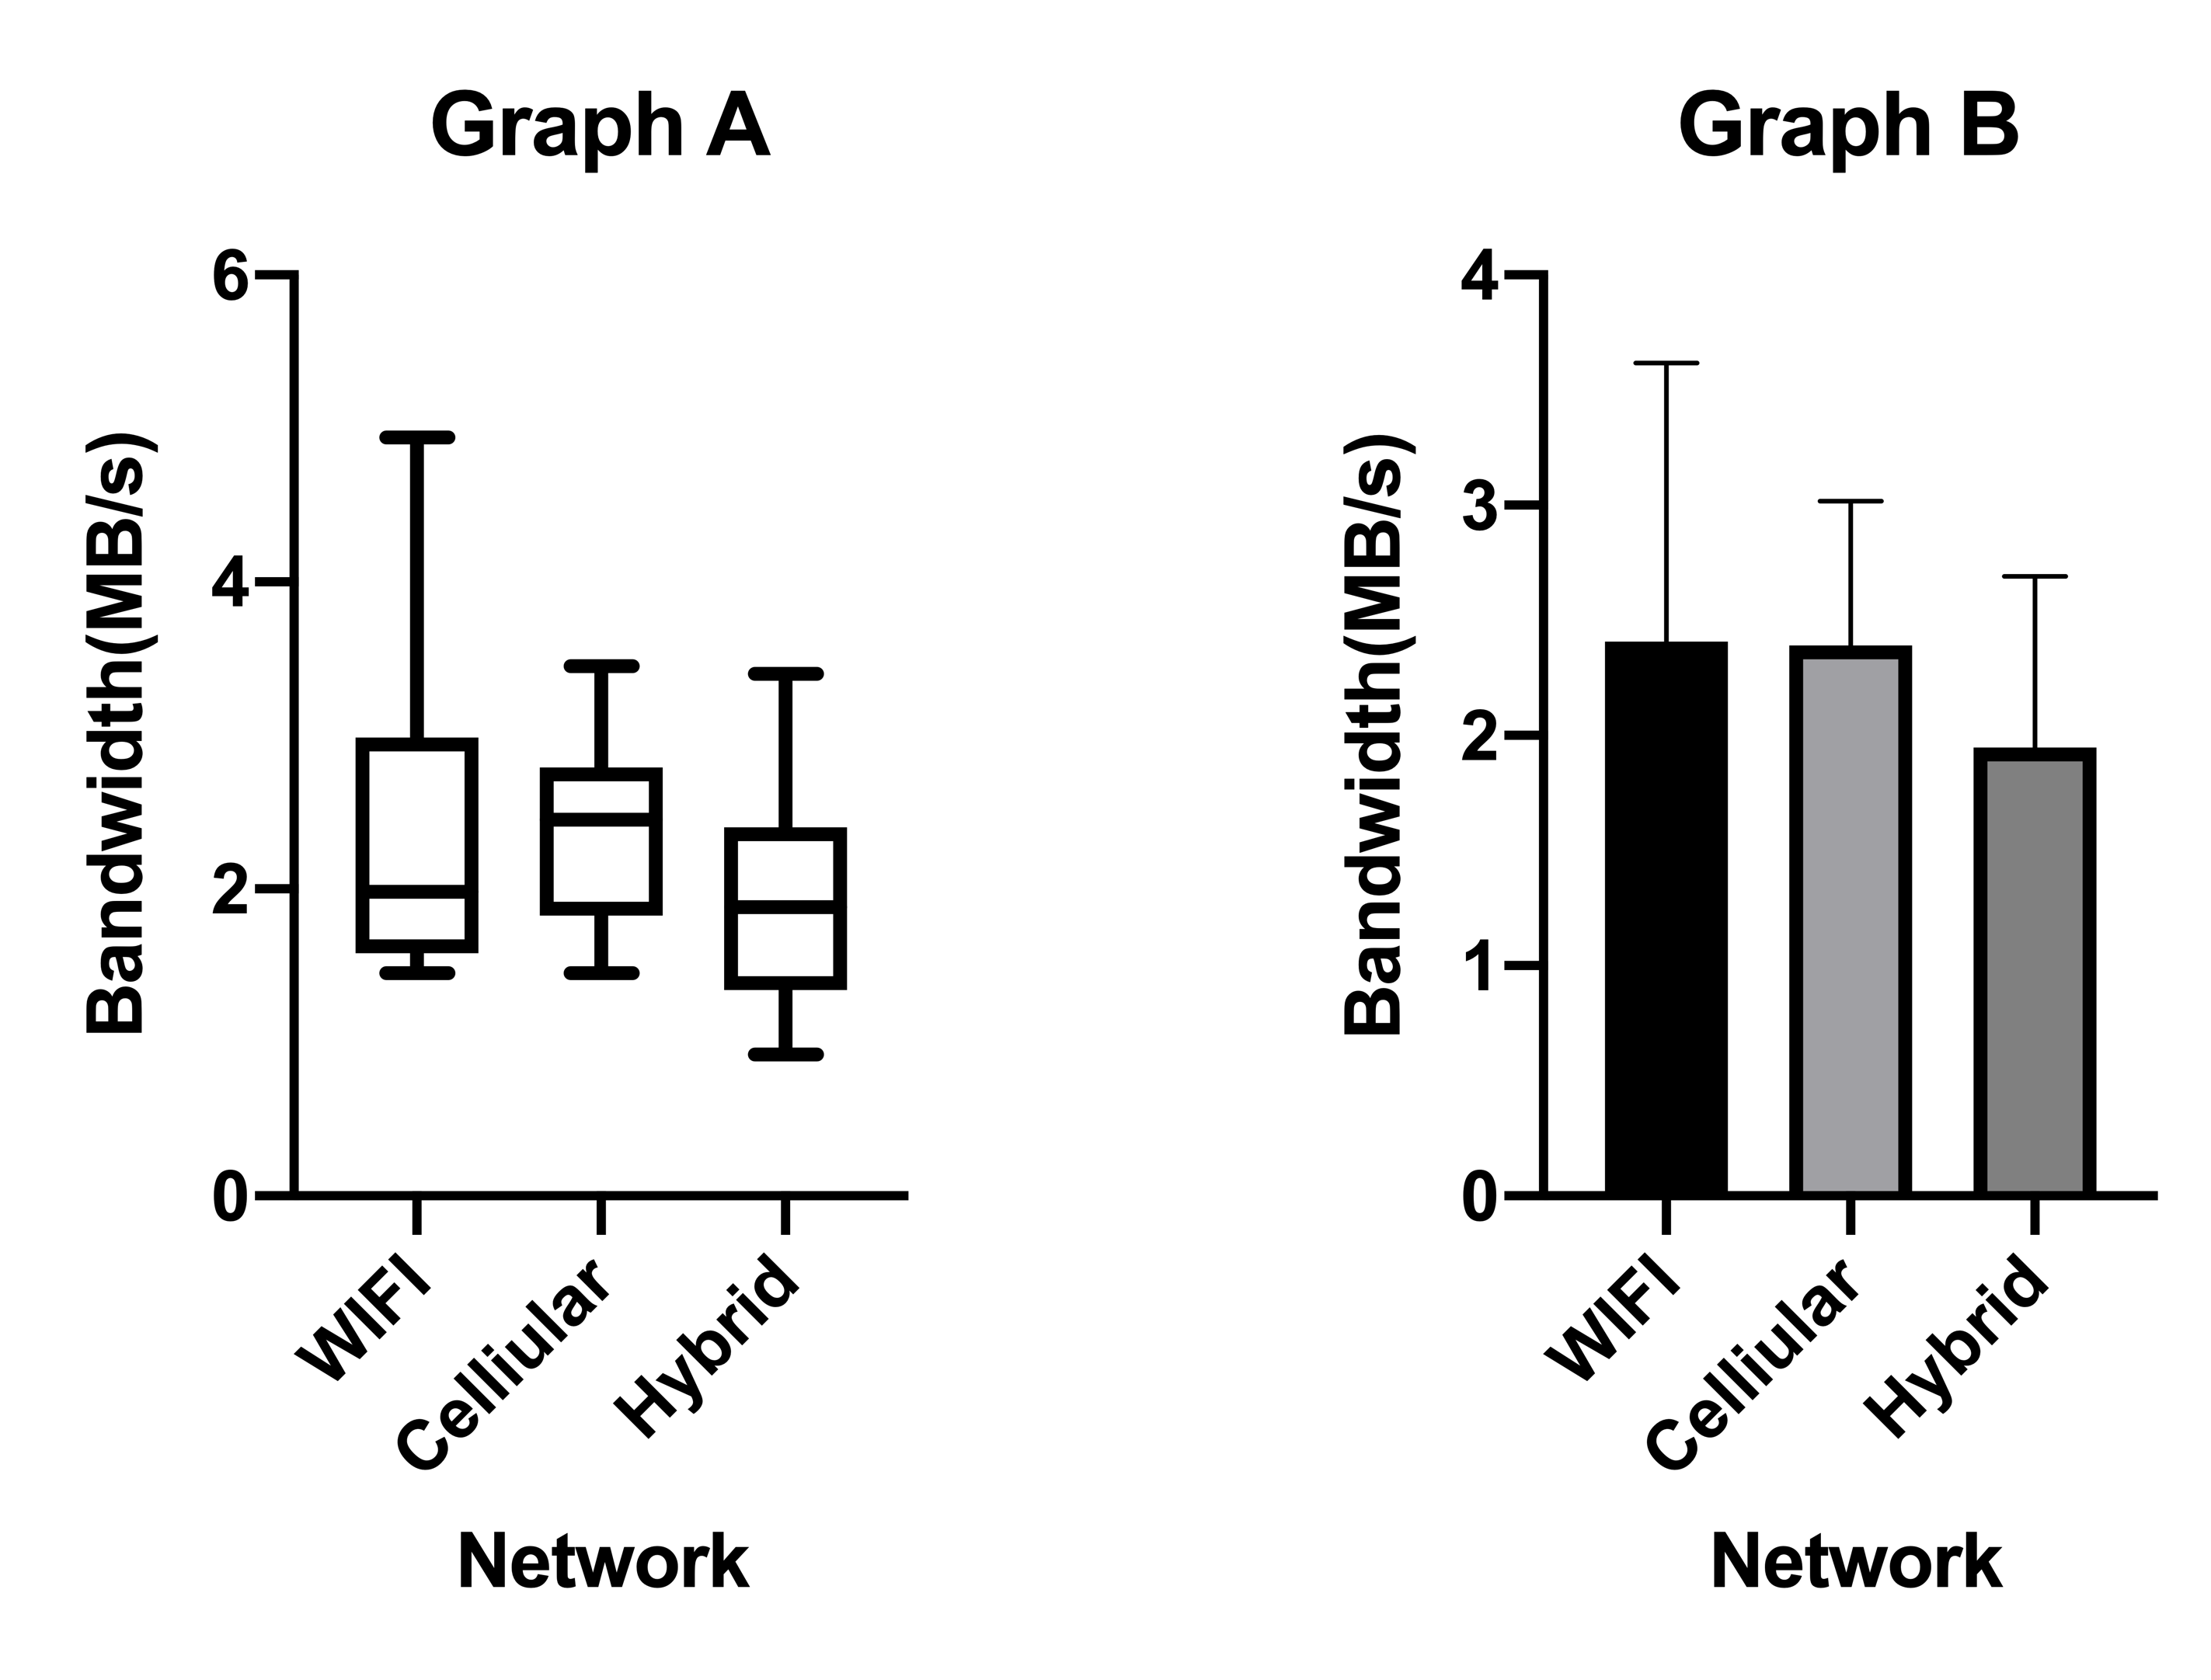
\includegraphics[scale=0.4]{graph_1_1}
    \caption{Available Bandwidth for different Networks }
    \label{fig:pca_coeff_fsf_gujnmk_z}
\end{figure}
\vspace{12pt}

As you can see in Figure \ref{fig:pca_coeff_fsf_gujnmk_z} WIFI network has the highest bandwidth when compared with the other networks. This is because it has the highest Radio frequency range form the above three wireless networks. Cellular network performance is generally stable than the other two networks. The highest mean value further justifies this argument. According to the graph, the hybrid network has relatively similar bandwidth to that of the cellular and WIFI networks.

%\begin{figure}[H]
%    \centering
%    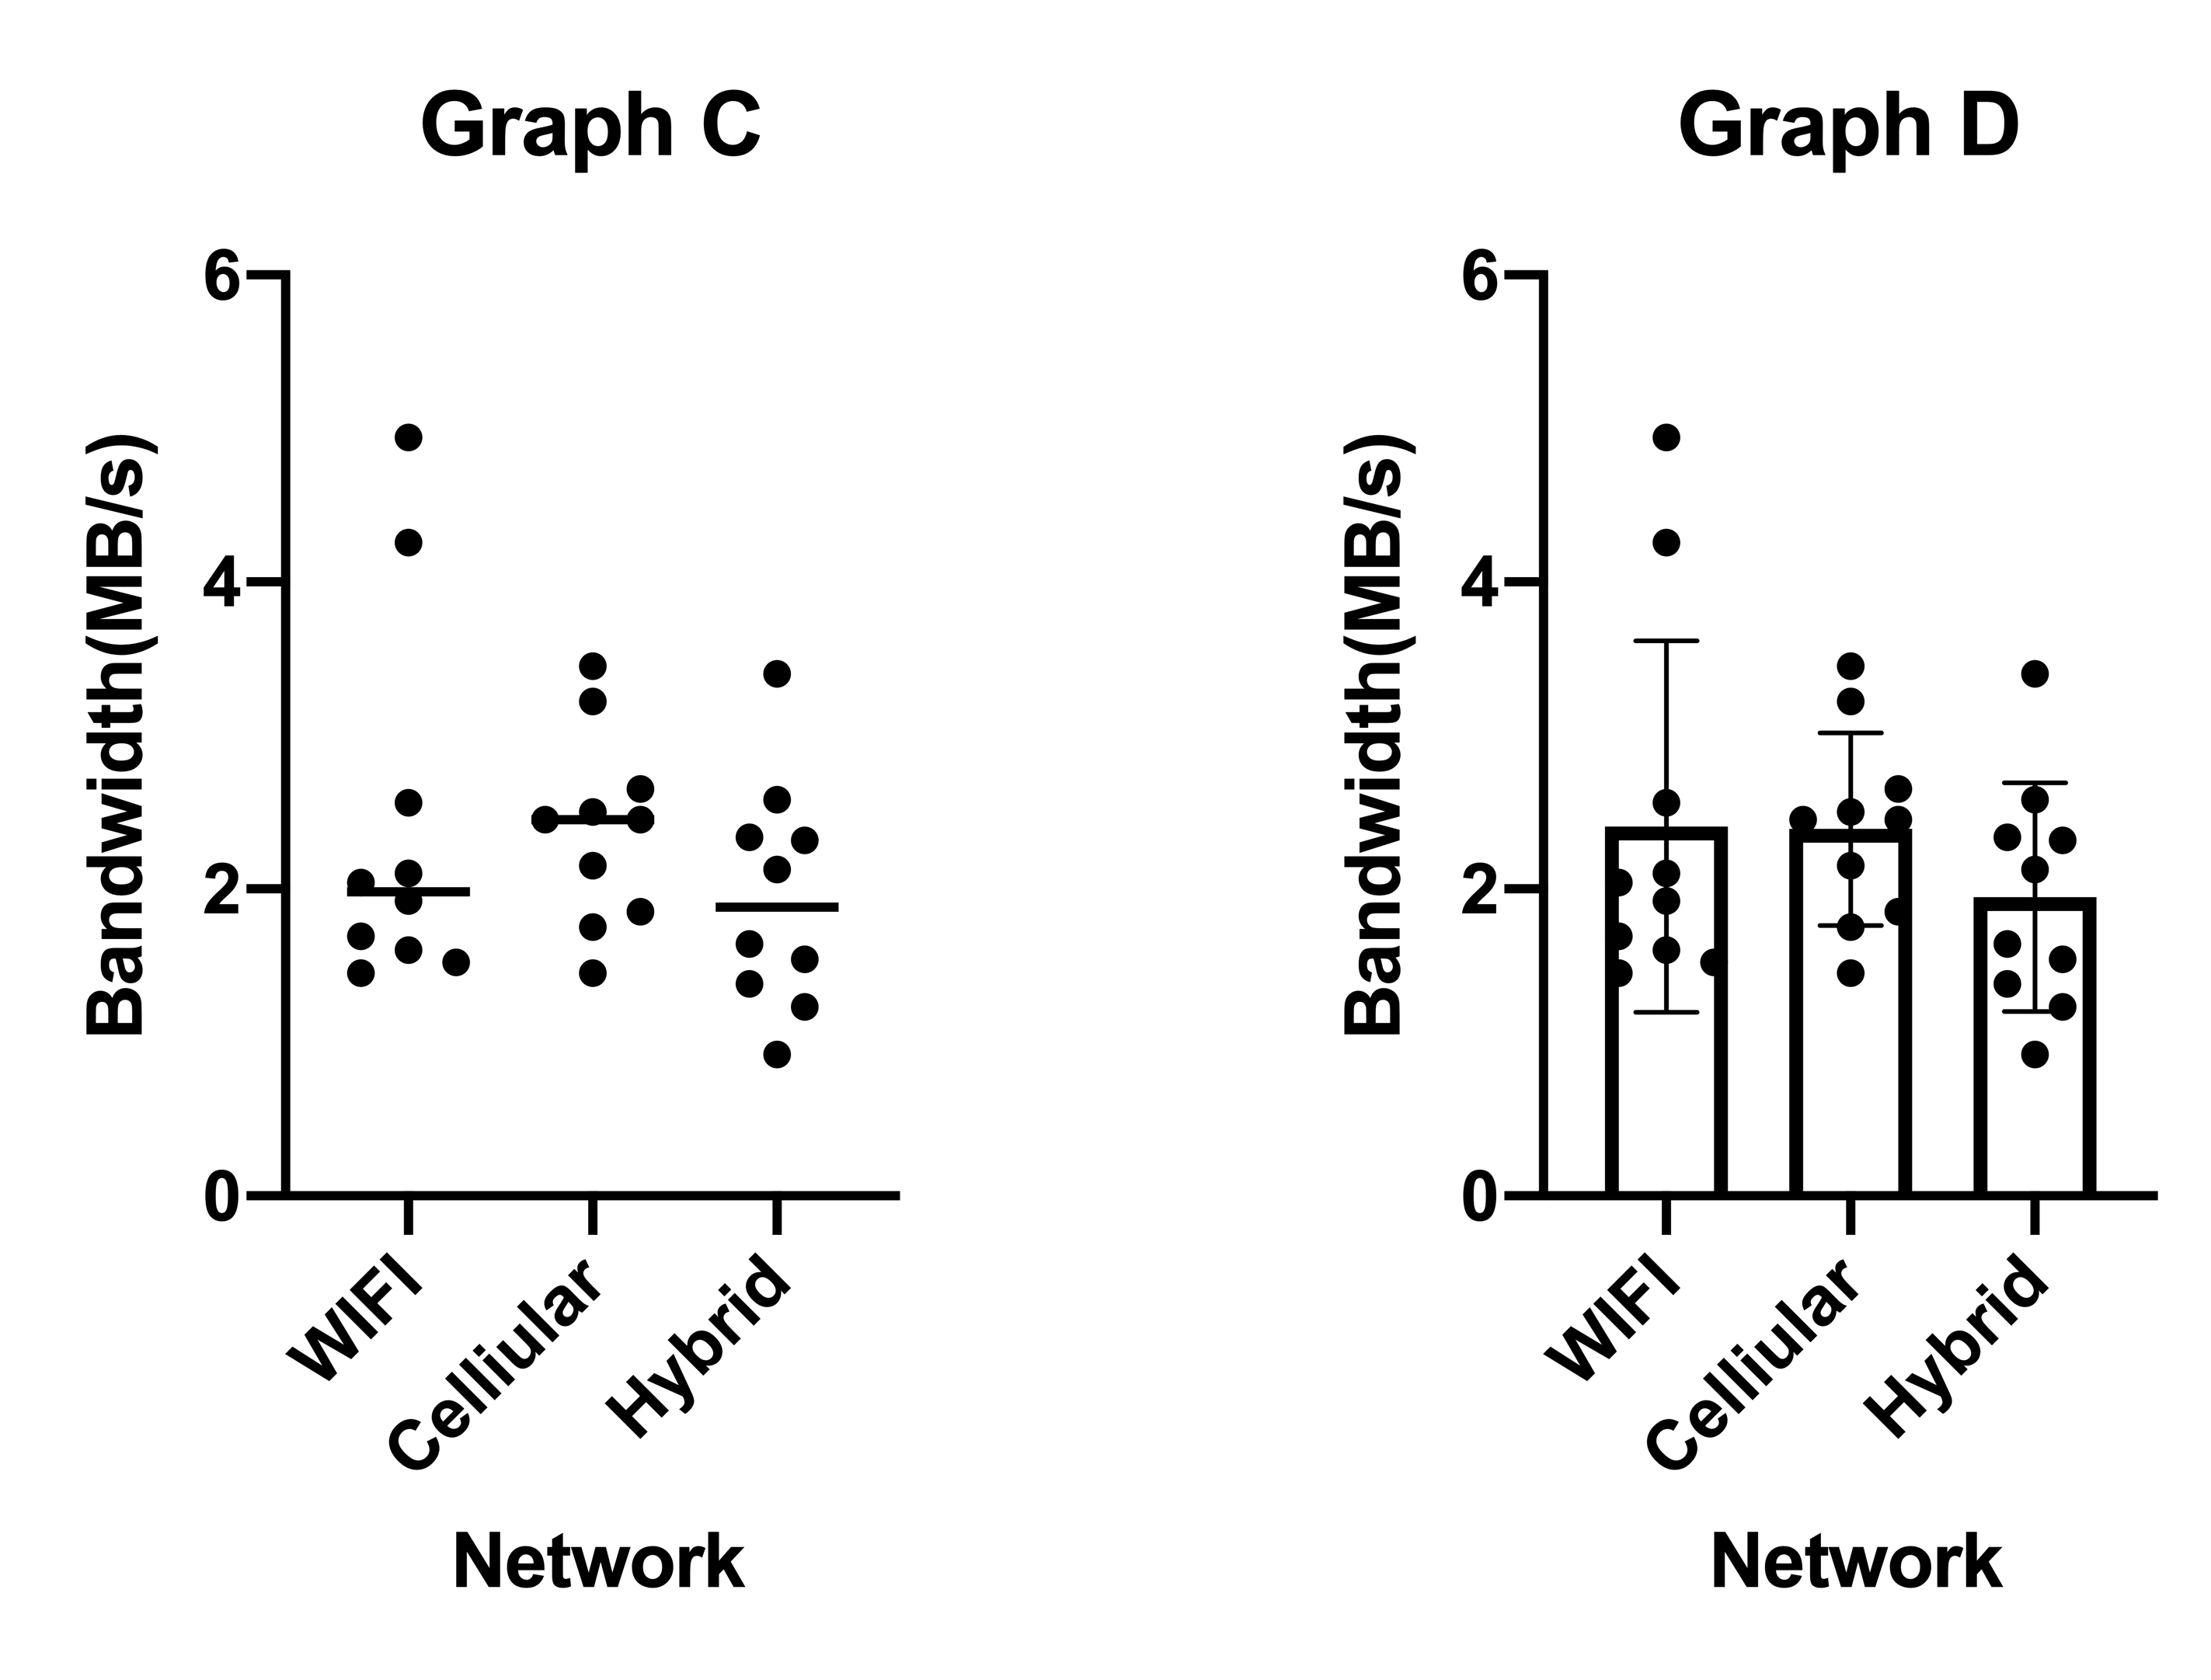
\includegraphics[scale=0.4]{graph_1_2}
%    \caption{Flow of the Constructive Research Design }
%    \label{fig:pca_kgkgk_fkkfkf_USNKGcoeff_z}
%\end{figure}
%\vspace{12pt}


\begin{figure}[H]
    \centering
    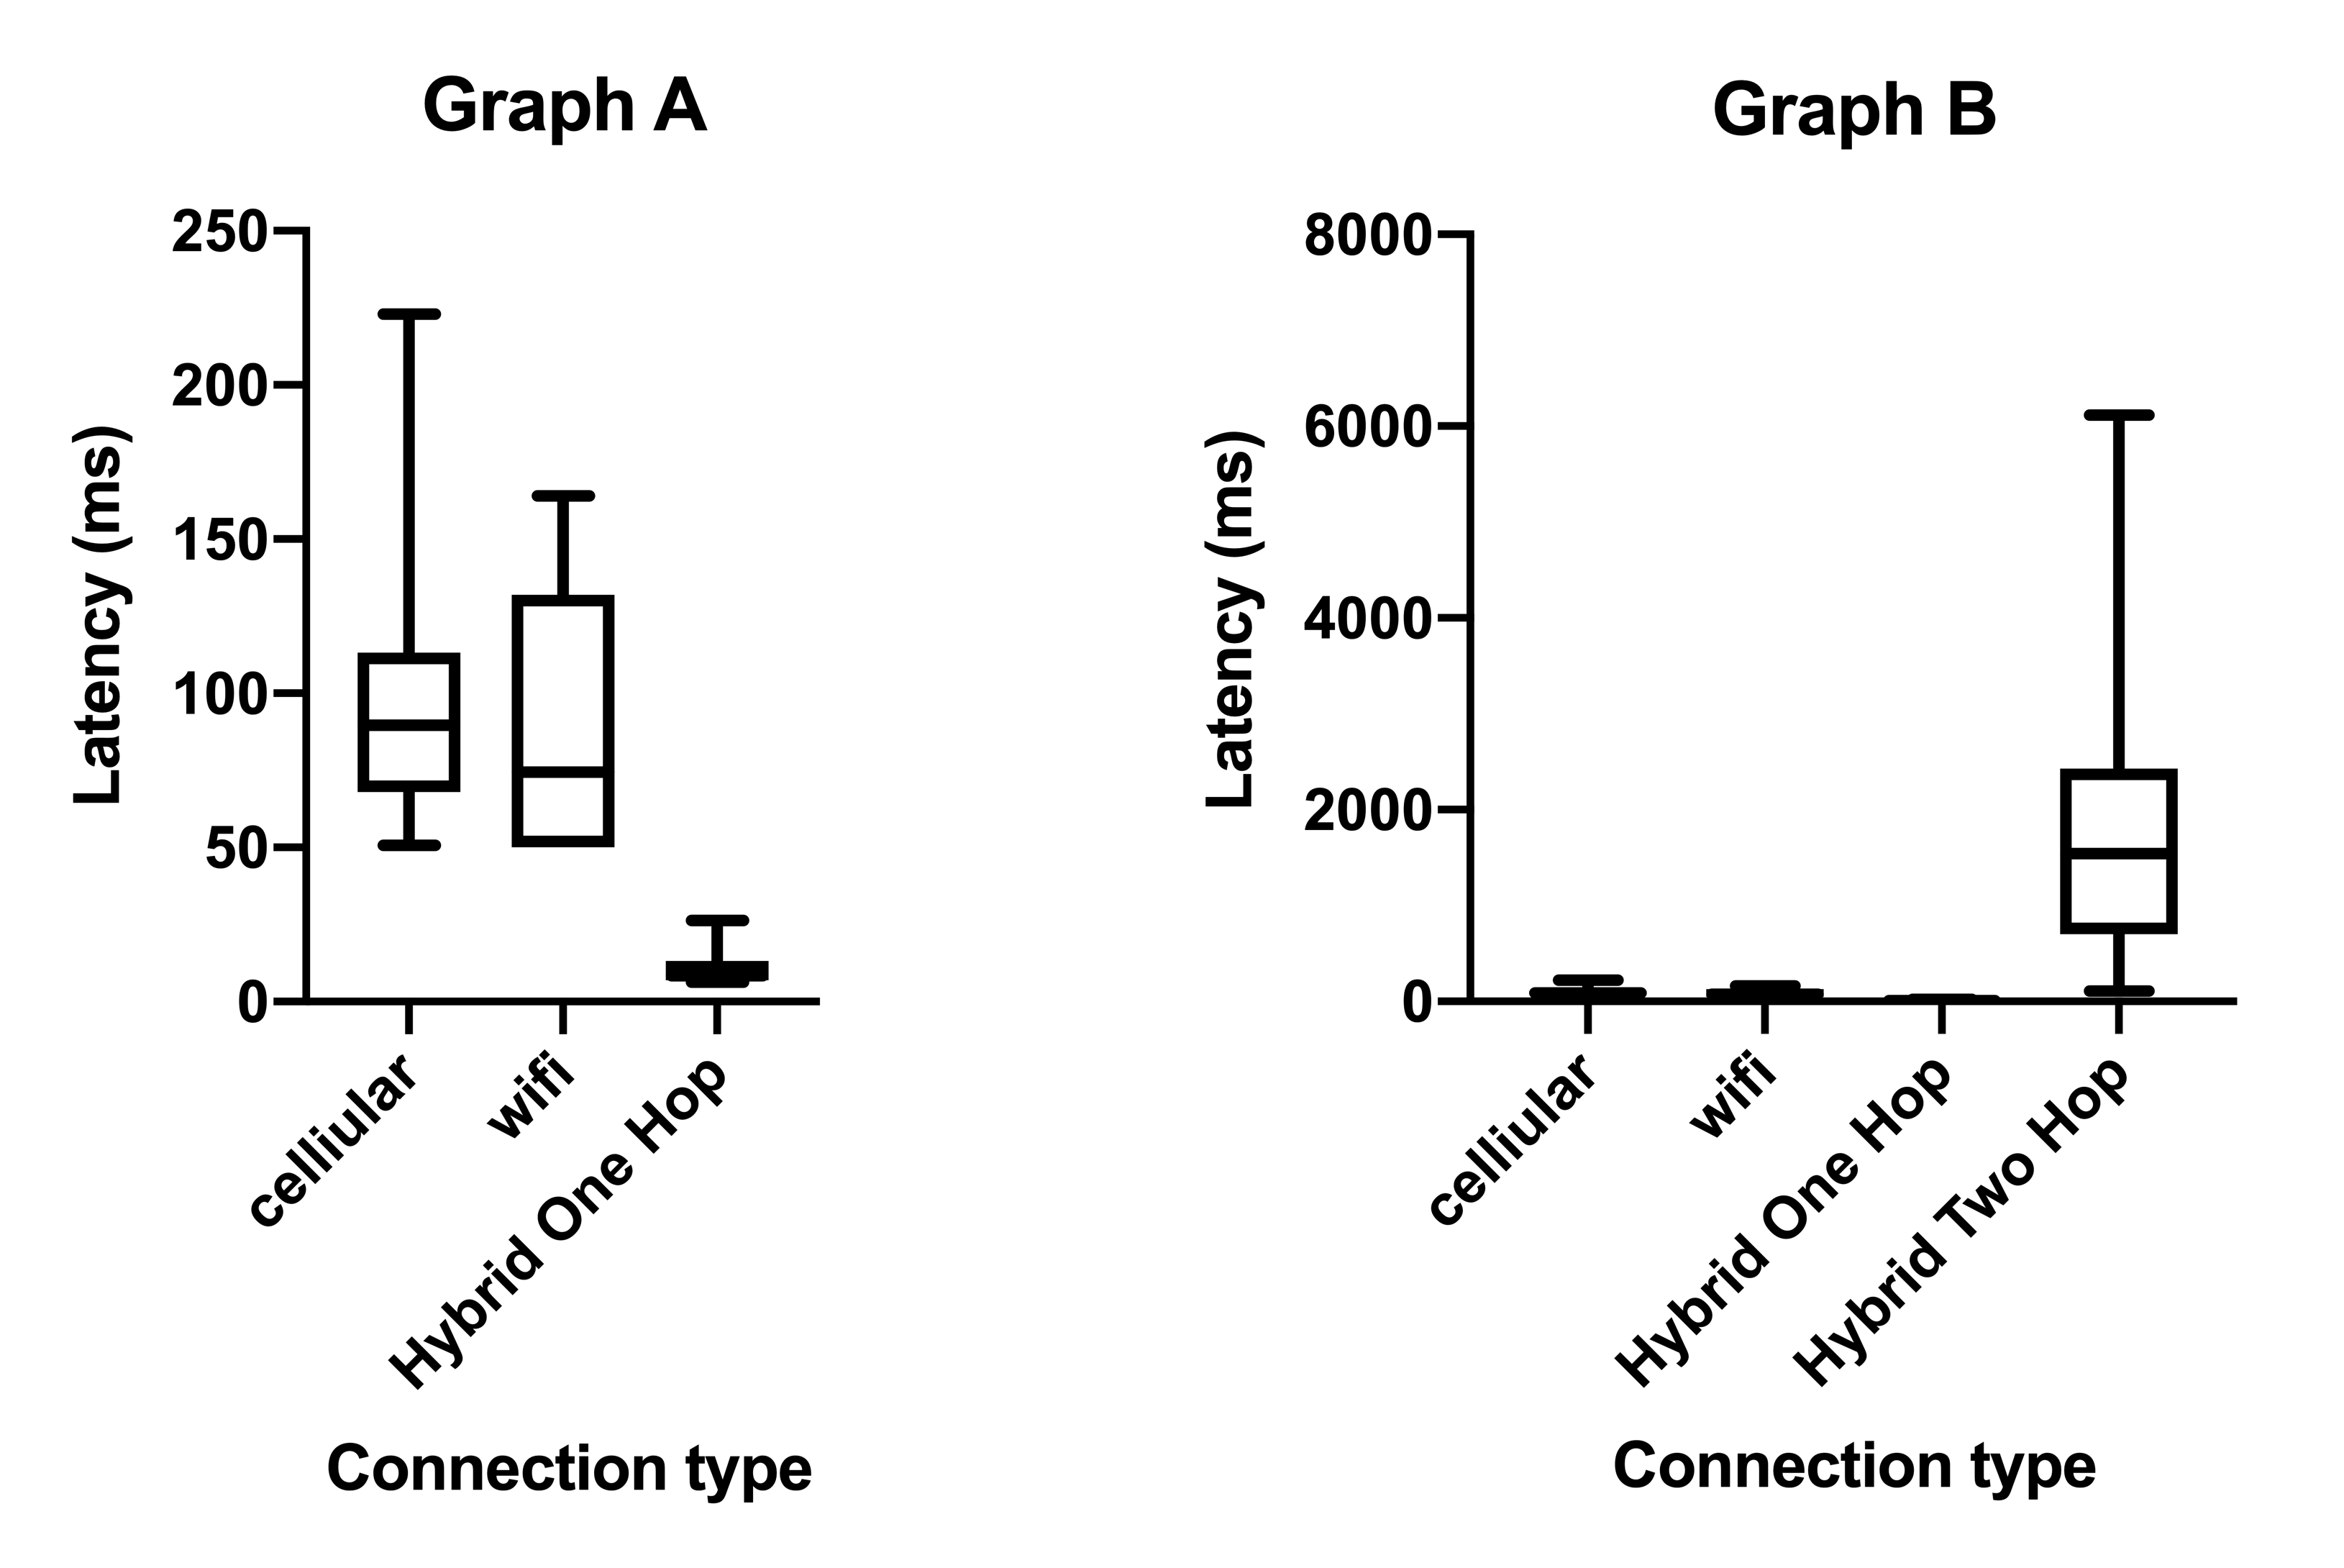
\includegraphics[scale=0.4]{Latency_of_network}
    \caption{Latency of Different Networks }
    \label{fig:pca_coeff_gfkfkkf_dkskk_sksksk_KKK_z}
\end{figure}
\vspace{12pt}

Due to being a peer to peer network, the hybrid network has the smallest latency from these two networks. So this is an improvement form the already available solutions. But when we increase the no of hops in the network this advantage diminishes rapidly. This can be seen by analyzing Figure \ref{fig:pca_coeff_gfkfkkf_dkskk_sksksk_KKK_z} graph A and graph B.

\begin{figure}[H]
    \centering
    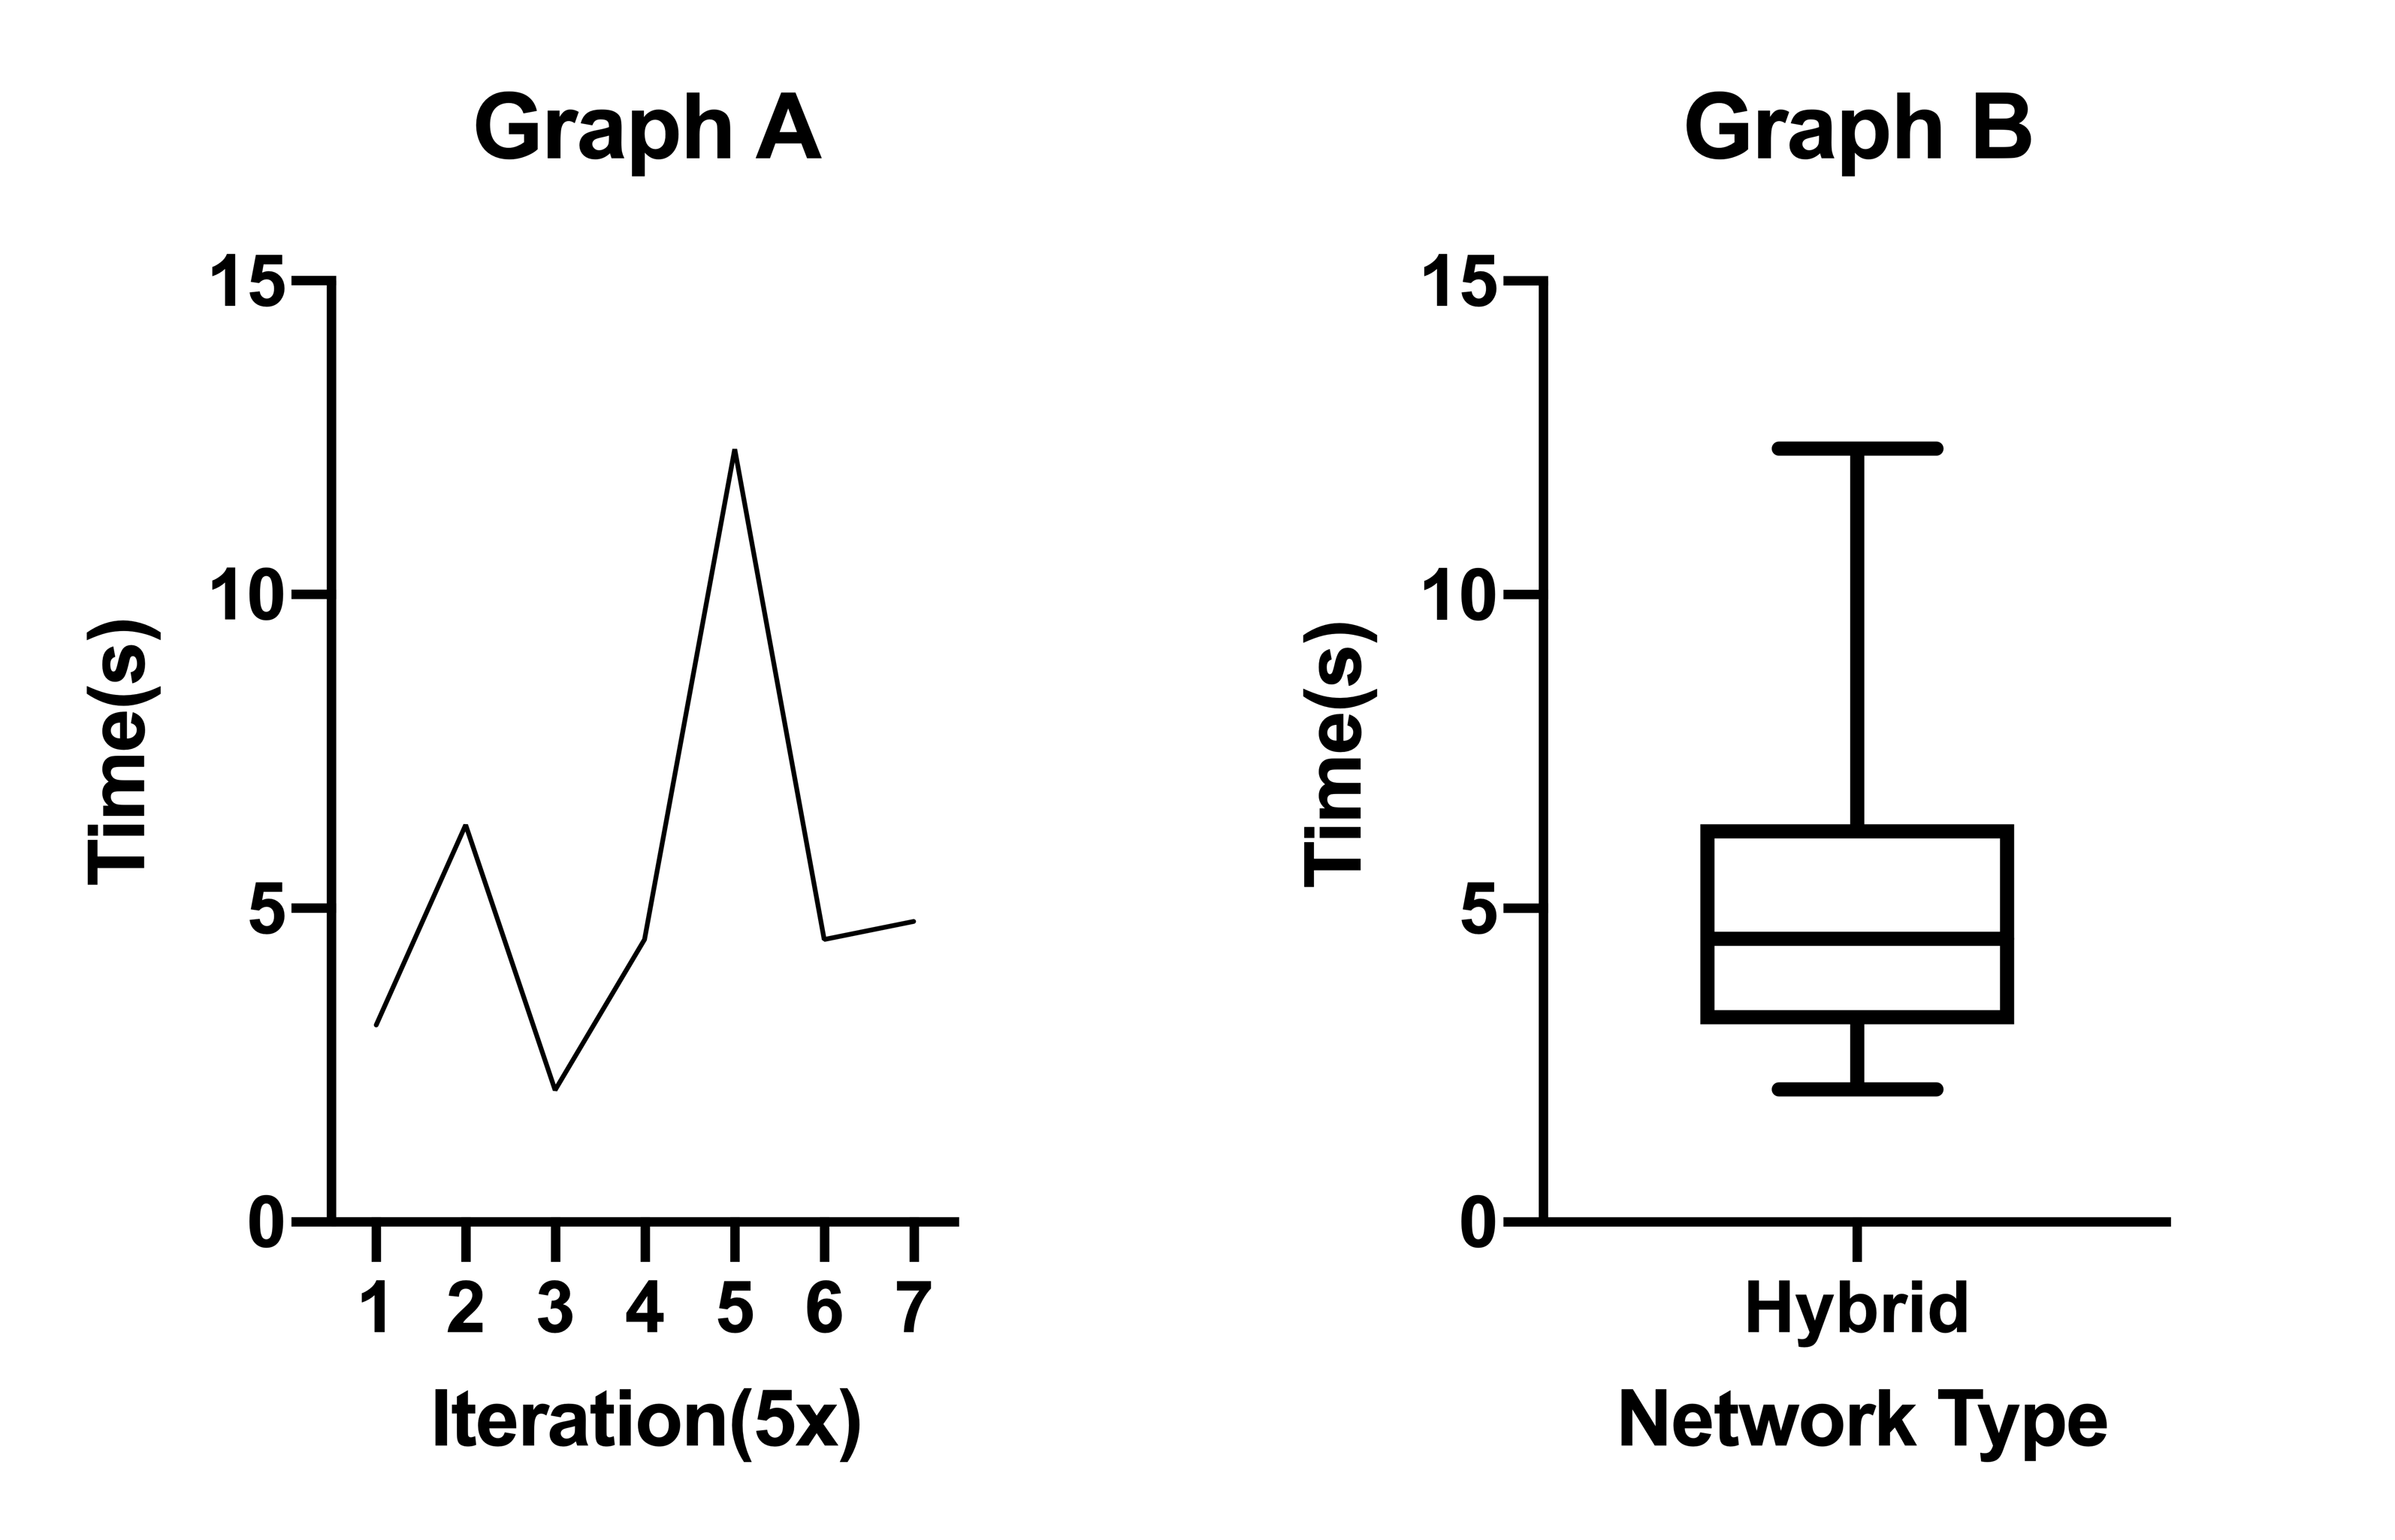
\includegraphics[scale=0.4]{time_to_switch_hybrid}
    \caption{Time takes for the Hybrid Network to do network Switching }
    \label{fig:pca_coeffdkgkdg_fmnkmnfg_kkfkf_fnfn_z}
\end{figure}
\vspace{12pt}
As the proposed solution is a unique one we were unable to find a similar solution that could be used to benchmark this network switching parameter. According to Figure \ref{fig:pca_coeffdkgkdg_fmnkmnfg_kkfkf_fnfn_z} Graph A  the actual value for switching fluctuates for different scenarios but the  mean value for switching in the network is about 5 seconds when comparing the  Figure \ref{fig:pca_coeffdkgkdg_fmnkmnfg_kkfkf_fnfn_z} Graph B.


\begin{figure}[H]
    \centering
    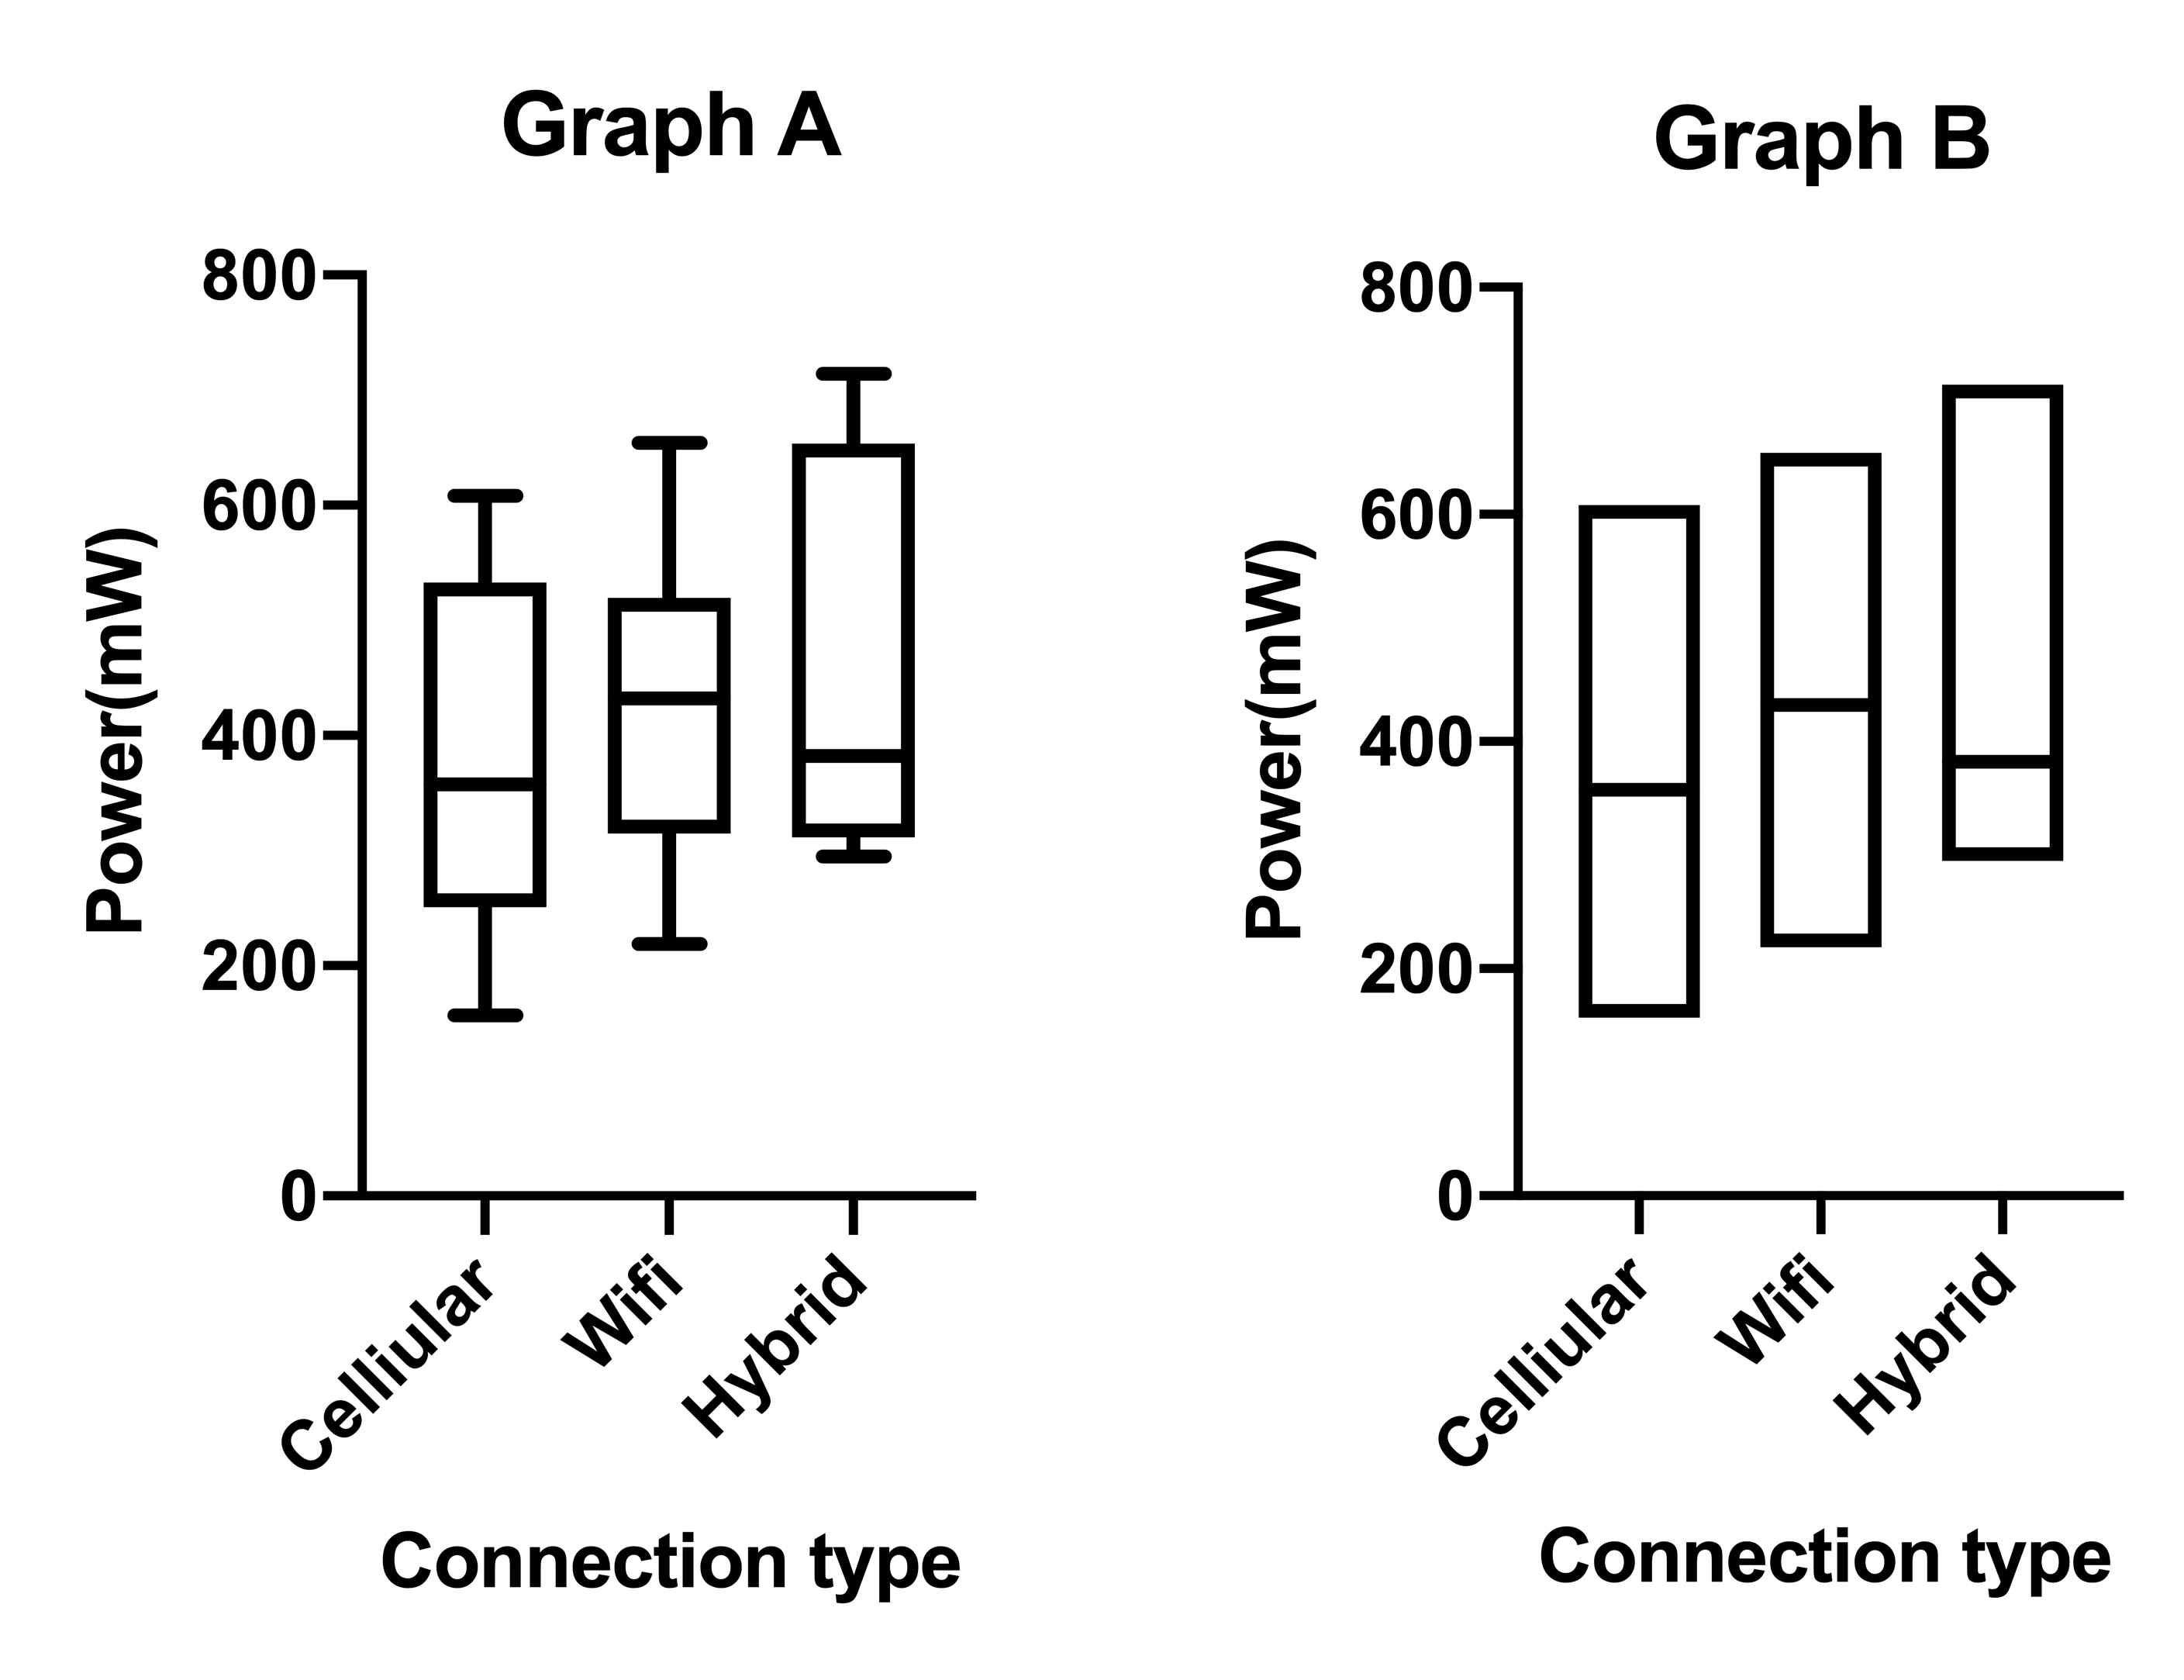
\includegraphics[scale=0.4]{power_draw.png}
    \caption{Power consumption of the particular Networks  }
    \label{fig:pca_coeff_ggjjgg_gjgjgj_jjggjz}
\end{figure}
\vspace{12pt}

When comparing the power consumption of the devices we used the internal battery power consumption measuring sensor to find the power consumption in real-time. As you can see in  Figure \ref{fig:pca_coeff_ggjjgg_gjgjgj_jjggjz} hybrid solution needs more power compared to the cellular and WIFI networks. This is due to the fact that it needs both of the above networks in order to function properly. As we use already available networking resources the extra layer of the protocol does not affect the energy consumption that considerably.










